% Report for the Solar Filament Segmentation Challenge 2026.
% Built on the organisers' Overleaf template: copy this file over main.tex of the template project,
% upload figures/*.pdf into a "figures" folder and extra.bib next to main.bib (both .bib files are read).
% Text that the template marks as "do not change" is kept verbatim.

\documentclass[sigconf]{acmart}
\input{preamble}

\guideStylefalse

\begin{document}

\title{A Native-Resolution U-Net Ensemble with a Metric-Tuned Instance Rule}
\subtitle{A Solution to the Solar Filament Segmentation Challenge 2026} % DO NOT CHANGE

\author{FIRSTNAME LASTNAME}   % <- TODO: your name
\affiliation{%
  \city{CITY}                 % <- TODO
  \country{Brazil}
}
\email{your.email@example.com} % <- TODO

\begin{abstract}
    This report describes our solution to the Solar Filament Segmentation Challenge~2026, a Kaggle competition on automatic segmentation of solar filaments in GONG H-$\alpha$ observations. We train two families of five U-Nets (ResNet-34 and ResNeXt-50 encoders) on full-resolution crops, using the fraction of annotators that marked each pixel as a soft target, and turn the averaged probability map into pixel-disjoint instances with a four-parameter rule chosen by directly maximising the pooled Panoptic Quality (PQ) on out-of-fold predictions. The pipeline reaches an out-of-fold PQ of $0.429$ (95\% interval $0.420$--$0.437$) and $0.38$ on the public leaderboard. We also quantify how much of the remaining gap is annotator disagreement rather than model error: two human annotators of the same frame score a PQ of only $0.34$ against each other, and the further attempts that we report as negative results did not move the score.
\end{abstract}

\maketitle

% ==================================== %
%              INTRODUCTION            %
% ==================================== %
\section{Introduction}
    This report goes over the details of our submitted solution to the Solar Filament Segmentation Challenge~2026 \cite{filament-segmentation-2026}. The challenge, launched on July~10,~2026, is organized by the Earth-Space AI Research (ESAIR) Lab\footnote{\href{https://www.esairlab.com/home}{www.esairlab.com/}}. This challenge utilizes the MAGFiLO dataset for evaluation of the segmentation algorithms \cite{ahmadzadeh2024dataset}.
    Our solution is deliberately simple: a semantic segmentation network, a connected-component step and one rule that decides which components are submitted. All design choices were made on out-of-fold predictions scored with our own implementation of the competition metric, and the public leaderboard was only used to confirm them. Code, weights and a notebook that regenerates the submission are public.\footnote{\url{https://github.com/zmickz/solar-filament-segmentation-2026}}

% ==================================== %
%              METHODOLOGY             %
% ==================================== %
\section{Methodology}\label{sec:methodology}

\begin{figure*}[t]
    \centering
    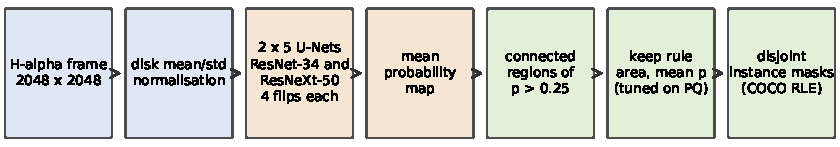
\includegraphics[width=\textwidth]{figures/pipeline.pdf}
    \caption{The inference pipeline. Blue: pre-processing; orange: the network ensemble; green: post-processing.}
    \label{fig:pipeline}
\end{figure*}

\subsection{Data and validation split}
    The training set has 707 frames of $2048\times2048$ pixels with 1{,}154 annotator records and 8{,}199 annotated filaments; 411 frames have one annotator, 145 have two and 151 have three. We split the frames into five folds \emph{by calendar date}, so that frames taken on the same day (often by different GONG stations, showing the same filaments) never sit on both sides of a split. Each fold model is trained on four folds and predicts the fifth; the union of those predictions (``out-of-fold'' maps) covers every training frame exactly once and is the only data used for model selection. The 180 test frames are never used for any choice.

\subsection{Pre-processing}
    A frame is read as 8-bit grayscale and standardised with the mean and standard deviation of the pixels inside the solar disk (radius 950 pixels). This removes the exposure differences between stations and years without any learned component. No resizing is done: thin filaments and barbs are a few pixels wide and do not survive down-sampling.

\subsection{Network and training}
    We use a U-Net \cite{ronneberger2015unet} whose encoder is an ImageNet-pretrained ResNet-34 \cite{he2016resnet} or ResNeXt-50 32x4d \cite{xie2017resnext} with a single input channel, and a plain decoder of four up-sampling blocks (two $3\times3$ convolutions each; 256, 128, 64 and 32 channels) with skip connections, giving one logit per input pixel (24 M and 32 M parameters). The two encoders give two families of five fold models, trained with the same script.

    \textbf{Soft target.} Where several annotators labelled a frame, the target of a pixel is the \emph{fraction of annotators} that included it in a filament, rather than a union or an intersection. The loss is binary cross-entropy plus soft Dice on this target. The network therefore learns to output a degree of agreement, which the post-processing uses below.

    \textbf{Sampling.} Training crops are $640\times640$ pixels taken at a random scale in $[0.8, 1.25]$; half of them are centred near a randomly chosen filament pixel, the other half are uniform over the frame. Augmentations are 90-degree rotations, flips and a mild brightness/contrast jitter. We train with AdamW \cite{loshchilov2019adamw} (learning rate $5\times10^{-4}$, weight decay $10^{-4}$, batch 8, 300 warm-up iterations, cosine decay) under mixed precision for a fixed budget of 40 minutes per fold (55 for ResNeXt-50) on one Tesla~T4, i.e.\ 8{,}100--9{,}200 iterations for ResNet-34. The two five-fold runs, including all predictions, take 2~h~22~min and 3~h~11~min on two T4 GPUs.

\subsection{Inference and post-processing}
    Each of the ten models predicts the full frame in one pass, averaged over four flips; the five maps of each family are averaged, then the two family maps (Fig.~\ref{fig:pipeline}). Instances are the 8-connected regions of $p>t_{lo}$, which makes them pixel-disjoint by construction. A region is submitted if its area is at least $a_{min}$, its mean probability at least $\bar p_{min}$ and its peak probability at least $t_{hi}$.

    \textbf{Tuning the rule on the metric.} The competition metric pools matches over all annotator records, $PQ=\sum_{TP} IoU / (TP + \tfrac12 FP + \tfrac12 FN)$. Submitting one more region always adds $\tfrac12$ to the denominator, and adds its IoU to the numerator only if it matches; a region is therefore worth submitting only when its expected matched IoU exceeds $PQ/2\approx0.21$. Pixel-level losses do not see this trade-off, so we choose $(t_{lo}, t_{hi}, a_{min}, \bar p_{min})$ by exhaustive search, scoring the out-of-fold maps with the pooled PQ (475 combinations for the ResNet-34 family, re-checked on 96 combinations for the final ensemble). The selected rule is $t_{lo}=0.25$, $a_{min}=320$~px, $\bar p_{min}=0.83$ ($t_{hi}$ has no measurable effect; $a_{min}=260$ ties). The low pixel threshold keeps the full extent of a filament, while the high mean-probability requirement removes regions on which the annotators, and hence the soft-target network, are undecided. On the test set this yields 1{,}201 filaments on 177 of the 180 frames. Figure~\ref{fig:examples} shows typical results.

\begin{figure}[t]
    \centering
    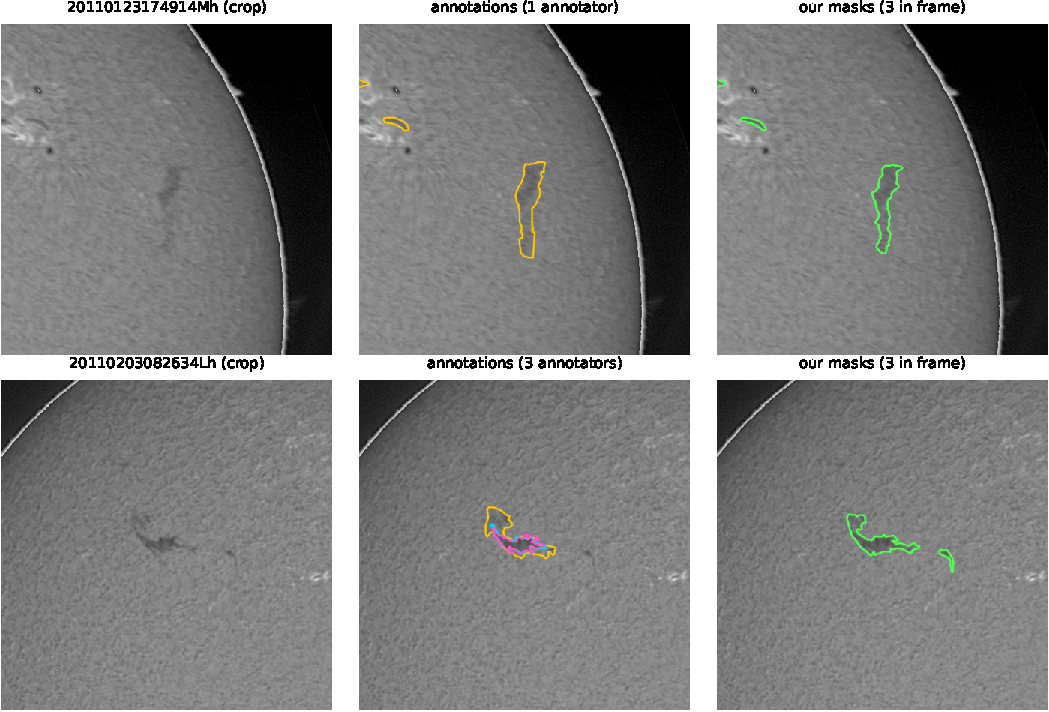
\includegraphics[width=\columnwidth]{figures/examples.pdf}
    \caption{Two training frames with their out-of-fold prediction. Left: input crop. Middle: human annotations, one colour per annotator. Right: our instance masks.}
    \label{fig:examples}
\end{figure}

% ==================================== %
%              EVALUATION              %
% ==================================== %
\section{Evaluation}\label{sec:evaluation}

\subsection{Strategy}
    All numbers are computed on the out-of-fold maps with our implementation of the pooled PQ, which we checked against a brute-force computation. Uncertainty is reported in two ways: a 95\% bootstrap interval obtained by resampling frames with replacement (1{,}000 resamples), and the spread across the five folds.

\subsection{Results}
\begin{table}[t]
    \caption{Out-of-fold results on the 707 training frames (8{,}199 annotated filaments; 4{,}998 predicted).}
    \label{tab:results}
    \begin{tabular}{lr}
        \toprule
        Quantity & Value \\
        \midrule
        PQ, pooled (95\% bootstrap interval) & 0.429 (0.420--0.437) \\
        PQ, mean $\pm$ std over the five folds & 0.429 $\pm$ 0.008 \\
        Segmentation quality (mean IoU of matches) & 0.679 \\
        Recognition quality (F1 of matches) & 0.632 \\
        TP / FP / FN & 5{,}178 / 3{,}007 / 3{,}021 \\
        IoU of matched filaments, 10/50/90th percentile & 0.56 / 0.68 / 0.79 \\
        Dice of matched filaments, median & 0.81 \\
        PQ on frames with 1 / 2 / 3 annotators & 0.432 / 0.442 / 0.418 \\
        Annotated filaments covered by several masks & 345 \\
        Masks covering several annotated filaments & 148 \\
        \midrule
        Public leaderboard PQ & 0.38 \\
        \bottomrule
    \end{tabular}
\end{table}

    Table~\ref{tab:results} and Fig.~\ref{fig:evaluation} summarise the performance. Fragmentation is limited: 345 annotated filaments (4\%) are covered by more than one of our masks, and 148 of our masks span more than one annotated filament.

\begin{figure*}[t]
    \centering
    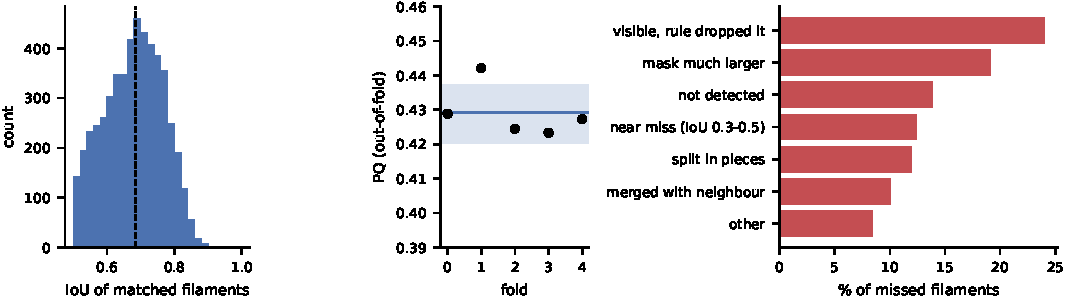
\includegraphics[width=\textwidth]{figures/evaluation.pdf}
    \caption{Left: IoU of the matched filaments (dashed: median). Middle: PQ of each fold (dots), pooled PQ (line) and its 95\% bootstrap interval (band). Right: why annotated filaments were missed.}
    \label{fig:evaluation}
\end{figure*}

\subsection{How much of the gap is label disagreement}
    We scored the annotators against each other with the same metric. Using one annotator's record as the prediction for another annotator of the same frame gives $PQ=0.34$, below our model. Even a perfect copy of one annotator would score only 0.68 on two-annotator frames and 0.55 on three-annotator frames, because every record is a separate ground truth. On our own probability maps, an oracle that keeps exactly the regions that match would reach 0.52 with the same regions, against 0.43 for our rule. A large part of what separates the model from a perfect score is therefore the question of \emph{which} dark structures a given annotator chose to mark, not where their boundaries are.

\subsection{Ablations and negative results}
    We report what did and did not help, because it narrows down where improvement can come from.
    (i)~\emph{A learned selector.} We built a tree of nested candidate regions per frame (thresholds 0.80/0.50/0.25 and three morphological closings that bridge gaps), trained a gradient-boosted regressor to predict each candidate's expected matched IoU from shape and confidence features, and selected the PQ-optimal disjoint set by exact dynamic programming on the tree. On the ResNet-34 maps its out-of-fold PQ is 0.428, against 0.424 for the four-parameter rule, while the oracle on the same tree is 0.557. Shape and confidence do not predict whether an annotator marks a structure.
    (ii)~\emph{A larger encoder alone.} The ResNeXt-50 family on its own reaches 0.422, against 0.424 for ResNet-34.
    (iii)~\emph{Ensembling both} (final solution). Averaging the two families gives 0.429 out of fold (better in four of the five folds) and raises the public score from 0.37 to 0.38. The gain is small and within the bootstrap interval, and it costs a second family of models; we keep it because the out-of-fold and public scores agree on it.
    (iv)~\emph{A stricter rule.} Since the public score is lower than the out-of-fold score, we tested whether the test set is annotated more sparsely by raising $\bar p_{min}$ to 0.89 on the ResNet-34 maps (24\% fewer masks). It lost 0.008 out of fold and 0.01 on the public leaderboard, so we did not adopt it.

\subsection{Strengths, weaknesses and possible improvements}
    \textbf{Strengths.} The pipeline is simple and reasonably fast (the ResNet-34 family takes about 2.6~s per frame on one T4 with flips; the full ensemble about four minutes per frame on CPU; ten weight files, 553~MB), has four interpretable post-processing parameters, produces disjoint masks without any overlap resolution step, and its validation is leak-free with respect to observation date.

    \textbf{Weaknesses.} (a)~Of the missed filaments, 24\% were detected but rejected by the rule and 14\% were not detected at all; these are mostly faint or very small filaments (41\% of all annotated filaments are below 1{,}000 pixels). (b)~19\% were segmented much larger than annotated and 12\% were split into pieces: the annotators draw one contour around a fragmented filament, while a connected-component step returns the pieces. (c)~The public score is 0.05 below the out-of-fold score; other participants reported the same offset. A stricter rule did not recover it (item iv), and both scores moved together in every change we made, so the out-of-fold estimate ranks solutions correctly even if its level is optimistic.

    \textbf{Possible improvements.} Predicting an explicit grouping signal (for example a filament-spine or centre-offset head) would address (b), which thresholding and morphology could not. Conditioning the keep rule on the annotation style expected at test time, or evaluating against a consensus of annotators, would address most of the remaining false positives, 18\% of which were in fact marked by a different annotator of the same frame.

% ==================================== %
%            ACKNOWLEDGMENT            %
% ==================================== %
\section{Acknowledgment}\label{sec:acknowledgment}
    % Do not change
    The organization of the Filament Segmentation Challenge 2026 is partially supported by the U.S. National Science Foundation (NSF) under Grant No. 2209912 and 2433781, directorate for Computer and Information Science and Engineering (CSE), and Office of Advanced Cyberinfrastructure (OAC), and Grant No. 2511630, AST Division Of Astronomical Sciences and MPS Directorate for Mathematical and Physical Sciences.

    The Filament Segmentation Challenge 2026 is sponsored by the U.S. National Science Foundation (NSF) National Solar Observatory (NSO).

    This work utilizes GONG data obtained by the NSO Integrated Synoptic Program, managed by the National Solar Observatory, which is operated by the Association of Universities for Research in Astronomy (AURA), Inc. under a cooperative agreement with the National Science Foundation and with contribution from the National Oceanic and Atmospheric Administration. The GONG network of instruments is hosted by the Big Bear Solar Observatory, High Altitude Observatory, Learmonth Solar Observatory, Udaipur Solar Observatory, Instituto de Astrofísica de Canarias, and Cerro Tololo Interamerican Observatory.

\bibliographystyle{ACM-Reference-Format}
\bibliography{main,extra}

\end{document}
